	
	\tikzset{every picture/.style={line width=0.75pt}} %set default line width to 0.75pt        
	
	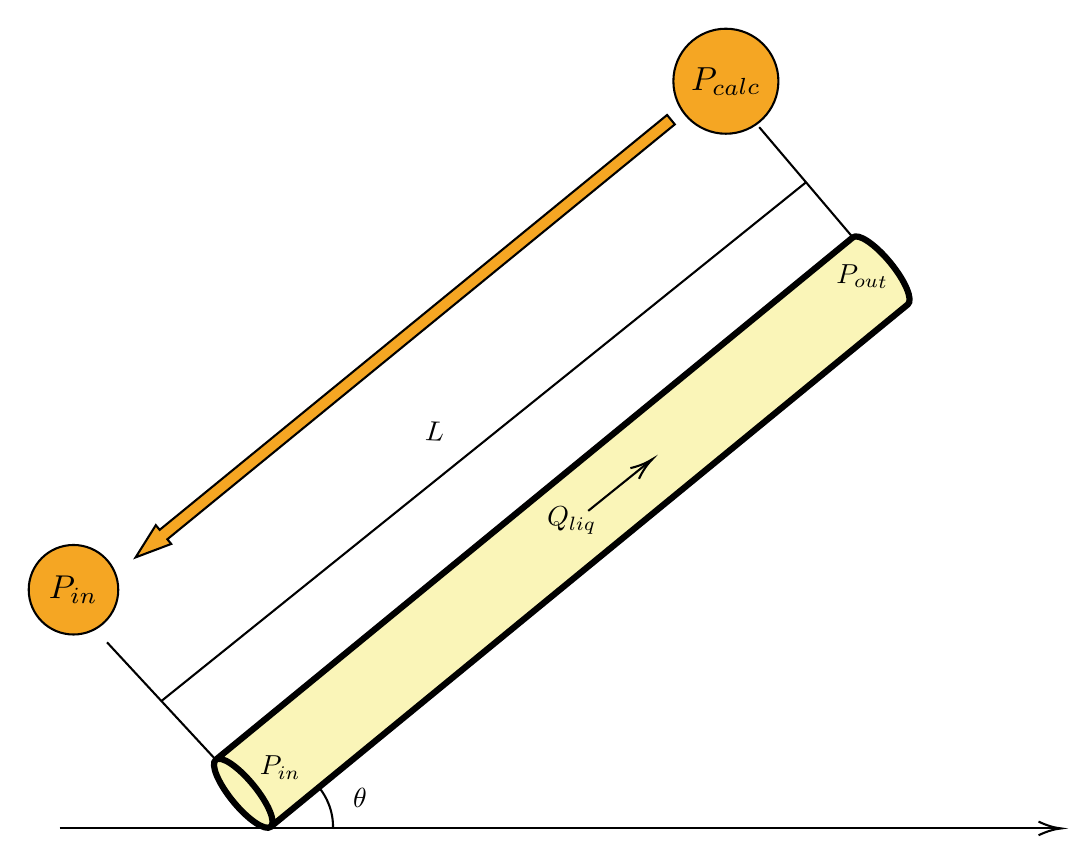
\begin{tikzpicture}[x=0.75pt,y=0.75pt,yscale=-1,xscale=1]
	%uncomment if require: \path (0,453); %set diagram left start at 0, and has height of 453
	
	%Shape: Can [id:dp7385102204739014] 
	\draw  [fill={rgb, 255:red, 250; green, 245; blue, 184 }  ,fill opacity=1 ][line width=2.25]  (198.23,370.28) -- (505.15,118.62) .. controls (507.82,116.43) and (515.92,121.88) .. (523.23,130.8) .. controls (530.54,139.72) and (534.3,148.72) .. (531.63,150.92) -- (224.71,402.57)(198.23,370.28) .. controls (200.9,368.08) and (209,373.54) .. (216.31,382.45) .. controls (223.63,391.37) and (227.39,400.38) .. (224.71,402.57) .. controls (222.03,404.77) and (213.94,399.32) .. (206.62,390.4) .. controls (199.31,381.48) and (195.55,372.47) .. (198.23,370.28) -- cycle ;
	%Shape: Arc [id:dp4602786709186524] 
	\draw  [draw opacity=0] (247.54,383.1) .. controls (249.72,385.66) and (251.51,388.62) .. (252.76,391.95) .. controls (254.22,395.8) and (254.84,399.77) .. (254.7,403.64) -- (224.71,402.57) -- cycle ; \draw   (247.54,383.1) .. controls (249.72,385.66) and (251.51,388.62) .. (252.76,391.95) .. controls (254.22,395.8) and (254.84,399.77) .. (254.7,403.64) ;
	%Straight Lines [id:da5353213855148988] 
	\draw    (145.83,313.7) -- (198.23,370.28) ;
	
	
	%Straight Lines [id:da6371642797081225] 
	\draw    (460.06,65.51) -- (505.15,118.62) ;
	
	
	%Straight Lines [id:da5708425902799406] 
	\draw    (172.03,341.99) -- (482.6,92.07) ;
	
	
	%Straight Lines [id:da5694938455522887] 
	\draw    (377.67,250.37) -- (407,226.74) ;
	\draw [shift={(408.56,225.48)}, rotate = 501.14] [color={rgb, 255:red, 0; green, 0; blue, 0 }  ][line width=0.75]    (10.93,-3.29) .. controls (6.95,-1.4) and (3.31,-0.3) .. (0,0) .. controls (3.31,0.3) and (6.95,1.4) .. (10.93,3.29)   ;
	
	%Straight Lines [id:da47656732513988986] 
	\draw    (123,403.37) -- (603.56,403.37) ;
	\draw [shift={(605.56,403.37)}, rotate = 180] [color={rgb, 255:red, 0; green, 0; blue, 0 }  ][line width=0.75]    (10.93,-3.29) .. controls (6.95,-1.4) and (3.31,-0.3) .. (0,0) .. controls (3.31,0.3) and (6.95,1.4) .. (10.93,3.29)   ;
	
	%Right Arrow [id:dp49730840239995544] 
	\draw  [fill={rgb, 255:red, 245; green, 166; blue, 35 }  ,fill opacity=1 ] (419.38,64.16) -- (174.9,264.05) -- (176.75,266.31) -- (159.61,272.77) -- (169.34,257.26) -- (171.19,259.52) -- (415.67,59.63) -- cycle ;
	
	% Text Node
	\draw (267.67,388.7) node   {$\theta $};
	% Text Node
	\draw (303.67,212.04) node [rotate=-2.44]  {$L$};
	% Text Node
	\draw (229.33,374.04) node [rotate=-0.74]  {$P_{in}$};
	% Text Node
	\draw (509.67,137.37) node [rotate=-0.74]  {$P_{out}$};
	% Text Node
	\draw (369.67,255.04) node [rotate=-0.61]  {$Q_{liq}$};
	% Text Node
	\draw  [color={rgb, 255:red, 0; green, 0; blue, 0 }  ,draw opacity=1 ][fill={rgb, 255:red, 245; green, 166; blue, 35 }  ,fill opacity=1 ]  (444, 43.37) circle [x radius= 25.3, y radius= 25.3]   ;
	\draw (444,43.37) node [scale=1.2,rotate=-359.71]  {$P_{calc}$};
	% Text Node
	\draw  [fill={rgb, 255:red, 245; green, 166; blue, 35 }  ,fill opacity=1 ]  (129.67, 288.37) circle [x radius= 21.57, y radius= 21.57]   ;
	\draw (129.67,288.37) node [scale=1.2,rotate=-0.74]  {$P_{in}$};
	
	
	\end{tikzpicture}